\begin{figure}[H]

    \caption{Nodo de marcador}

    \centering

    \setlength{\tabcolsep}{0pt}
    \renewcommand{\arraystretch}{1}

    \begin{tabular}{
    |>{\centering\arraybackslash}m{0.42\textwidth}|
    }
        \hline

        \rule{0pt}{0.02\textwidth}

        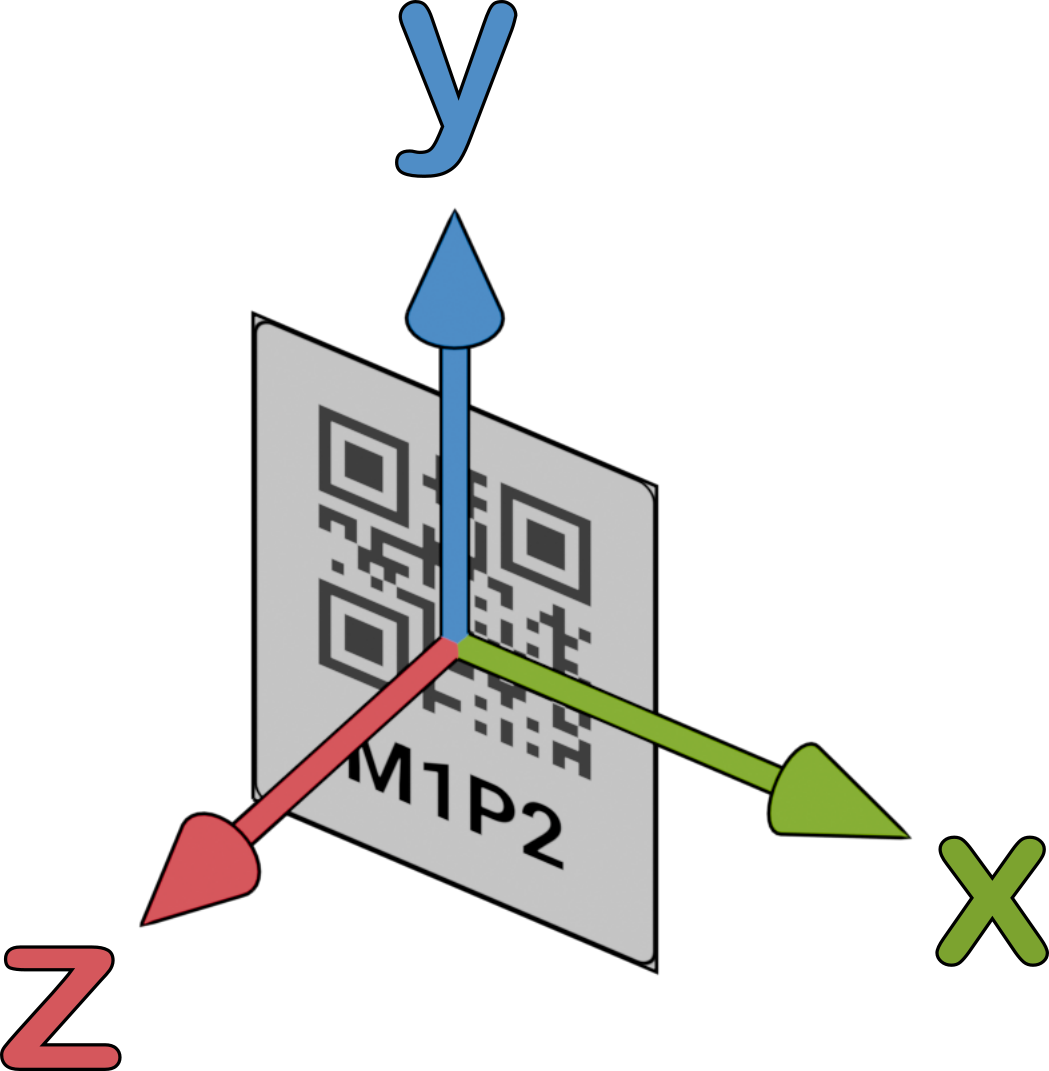
\includegraphics[width=0.38\textwidth]
        {assets/figures/second_phase/node/img_node_augmented_image.png}

        \\[0.04\textwidth] \hline

    \end{tabular}
    \label{fig:node_augmented_image}
    
    \caption*{\textit{Nota}. \textnormal{La imagen sólo ilustra la transformación detectada de un marcador físico, este nodo no añade un nodo de control de transformación (\textit{gizmo}).}}

\end{figure}
\fixvspace{0.5}